\documentclass[12pt,a4paper]{tufte-handout}
\usepackage{color} % for coloured text
\usepackage{listings} % for code listings
\usepackage{amsmath} % for math!
\usepackage{graphicx} % for pictures...
\usepackage{caption} % for margin figures
\usepackage{hyperref} % links
\usepackage{booktabs}
\usepackage{gensymb}
\usepackage{comment}
\usepackage[algo2e]{algorithm2e}
%\usepackage{algpseudocode}
\newcommand{\bdp}{\mathbf{\Delta p}}
\newcommand{\bSig}{\mathbf{\Sigma}}
\newcommand{\rT}{\mathrm{T}}
\newcommand{\bb}{\mathbf{b}}
\renewcommand{\bf}{\mathbf{f}}
\newcommand{\bp}{\mathbf{p}}
\newcommand{\br}{\mathbf{r}}
\newcommand{\bs}{\mathbf{s}}
\newcommand{\bt}{\mathbf{t}}
\newcommand{\bx}{\mathbf{x}}
\newcommand{\by}{\mathbf{y}}

\newcommand{\bA}{\mathbf{A}}
\newcommand{\bF}{\mathbf{F}}
\newcommand{\bI}{\mathbf{I}}
\newcommand{\bJ}{\mathbf{J}}
\newcommand{\bR}{\mathbf{R}}
\newcommand{\bS}{\mathbf{S}}
\newcommand{\bT}{\mathbf{T}}
\newcommand{\bX}{\mathbf{X}}

\newcommand{\inv}[1]{#1^{-1}}
\newcommand{\abs}[1]{\left\lvert #1\right\rvert}
\newcommand{\norm}[1]{\left\lvert\left\lvert #1\right\rvert\right\rvert}
\newcommand{\qmark}[1]{\mbox{}\hfill\textbf{[#1]}}
\newcommand{\argmin}{\operatorname*{arg\,min}}
\newcommand{\argmax}{\operatorname*{arg\,max}}
\newcommand{\var}{\operatorname*{var}}
\newcommand{\diag}{\operatorname*{diag}}
\newcommand{\tr}{\operatorname*{Tr}}
\newcommand{\dcos}{d_\mathrm{cos}}
\newcommand{\deuc}{d_\mathrm{euc}}
 % New commands
\usepackage{framed}
\lstset{
  language=matlab,
  basicstyle=\ttfamily,
  keywordstyle=\ttfamily
}

\setcounter{secnumdepth}{2}
\title{Computational Tools for Modelling and Analysis: Clustering}
\author{Dr Iain Styles}

\date{\today}

\begin{document}
%\Large\sffamily
\maketitle
\section{Introduction}

The dimensionality reduction techniques we studied in the previous section are effective tools for telling us about the bulk structure of a dataset (how many underlying dimensions it has, what the spread of points in each of the dimensions is), but they are not always able to tell us anything about the ``fine structure'' within the data. For example, in the top part of Figure~\ref{fig:simpleclusters}, the projections of this dataset onto principal component 1 would enable you to determine the presence of two distinct ``clusters'' of points in the data, whereas in the bottom part of the figure, they would not. The discovery of the clusters would likely tell us something in interesting about the data so we need some way of finding them. Clustering techniques aim to do just that: in essence, we aim to find groups of points that are in some way ``similar''. In this unit, we will examine a few different ways of finding clusters and the assumptions behind them.
\begin{marginfigure}
  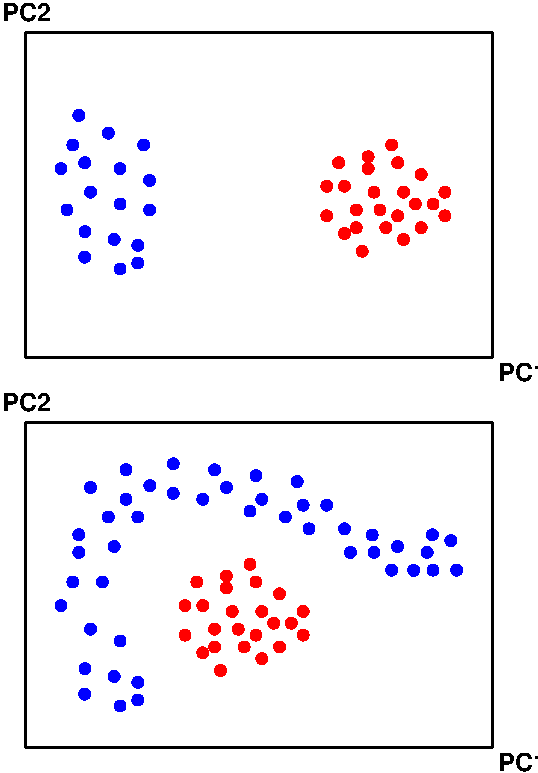
\includegraphics[width=\textwidth]{simpleclusters}
  \caption{Some simple clusters}
  \label{fig:simpleclusters}
\end{marginfigure}

\section{General Approaches to Clustering}
  There are many hundreds of clustering algorithms, all with different underlying assumptions about the nature of the data. For example, some assume that the members of each clusters are normally distributed. All methods are based on computing the ``similarity'' of points within the dataset: the outcome of all clustering algorithms is sets (groups) of points that are, by some measure, similar.

Assuming that we have a sensible definition of ``similar'', there are, roughly speaking, two main approaches that can be summarised as:
  \begin{itemize}
    \item Bottom-up clustering: starting with individual data points, group similar ones together until all points are in appropriate groups.
    \item Top-down clustering: starting with the whole data set, remove dissimilar points until all points are in appropriate groups.
  \end{itemize}

We will look at some examples of both of these methods, but we must first consider what we mean when we say the two data points are ``similar'' or otherwise.

\section{Measures of Similarity}

 All clustering techniques require some measure of similarity to be defined. There are two important factors to consider:

      \begin{itemize}
        \item What is the appropriate measure of similarity?
        \item How do you measure the similarity of groups of points?
      \end{itemize}

\subsection{Distances}
The first of these might seem like a rather trivial decision: we are all aware of one obvious measure of similarity, the standard \textbf{Euclidean distance} derived  trivially from Pythagoras' theorem. Given data points $\bx^{(1)}$ and $\bx^{(2)}$, this is defined as

\begin{equation}
  \deuc(\bx^{(1)},\bx^{(2)}) = \sqrt{\sum_{i=1}^M \left[x_i^{(1)} - x_i^{(2)}\right]^2}
\end{equation}

\begin{marginfigure}
  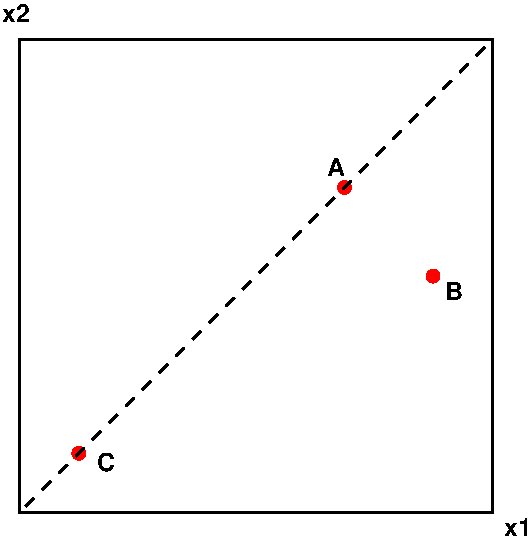
\includegraphics[width=\textwidth]{distances}
  \caption{Data points A and B are nearest neighbours in a Euclidean sense, but A and C could be said to be more ``similar''.}
  \label{fig:distances}
\end{marginfigure}

However, Euclidean distance does not necessarily capture the full range of ways in which two data points can be similar. In Figure~\ref{fig:distances} we show three data points, A, B and C. Clearly the two most similar points from a Euclidean perspective are A and B: they ae ``closest'' to each other. However, in a somewhat different sense, A could be regarded as being more similar to C than it is to B: A and C both lie on a straight line that goes through through the original, and hence the components of A are just a scalar multiple of the components of C (this is not the case for A and B). Adopting an analogy from colour science, we might regard C as being ``dark blue''. A is ``brighter (more intense) than C and is thus a lighter blue, whereas C, lying away from the line, is of a similar intensity to A but of a different hue (for example, a pale green). The Euclidean distance does not capture the similarity between A and C. One metric that does is the so-called \textbf{cosine distance}, than looks at the angle between two data points:

\begin{equation*}
  \dcos(\bx^{(1)},\bx^{(2)}) = \cos^{-1}\left(\frac{\bx^{(1)}\cdot\bx^{(2)}}{\norm{\bx^{(1)}}_2\norm{\bx^{(2)}}_2}\right)
\end{equation*}

In the example, the cosine distance between A and C would be zero, as both are at the same angle relative to the origin, thus this measure capture this similarity between the data points. The choice of similarity measure is highly dependent on the nature of your dataset. Other distance measures that can sometime be useful are the correlation, Manhattan and Mahalanobis distances.

\subsection{Normalisation}
The same considerations also lead us to consider ``normalising''  each item of data such that they have some common property. For example, we could normalise the points in Figure~\ref{fig:distances} such that all sample vectors have the same length: $\frac{1}{N}\sum_{i=1}^nx_i^2=1$. Normalisation removes global ``intensity'' differences from the data, and this type of normalisation brings points on the same radial lines together so that they can be clusters. When used with the Euclidean distance, this normalisation yields the same results as using the cosine distance. As always, whether it is sensible or necessary to normalise your data depends on the nature of the data.

\subsection{Linkage}
\begin{marginfigure}
  Single Linkage
  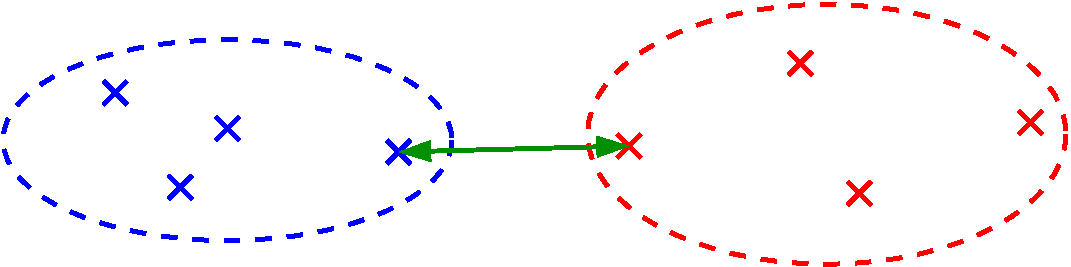
\includegraphics[width=\textwidth]{singlelinkage}
  \vskip 0.5cm
  Average Linkage
  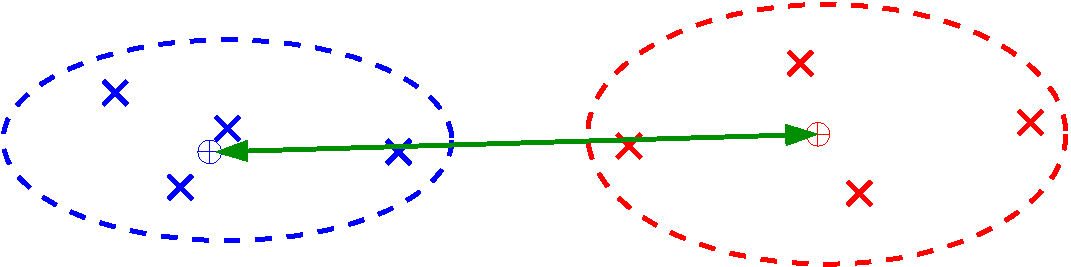
\includegraphics[width=\textwidth]{averagelinkage}
  \vskip 0.5cm
  Complete Linkage
  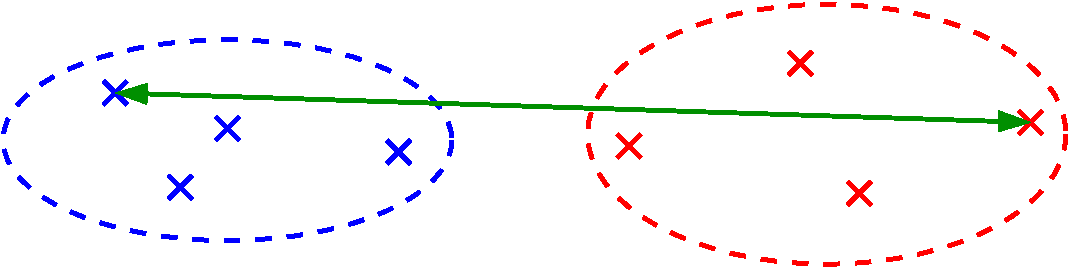
\includegraphics[width=\textwidth]{completelinkage}
  \caption{Linkage strategies for clustering of groups.}
  \label{fig:linkage}
\end{marginfigure}

The second issue is how we measure the similarity between groups. Let us imagine that we have established that that a pair of points (say A and B) belong together, whilst another pair of points (C and D) also belong together. Should we then group these pairs together? It is not at all clear how we should measure the similarity of these groups: should we measure from the edges of the groups, or from their centres, or from somewhere else? Again, the answer is that it depends on the dataset. There are three main strategies available for ``linkage'' (Figure~\ref{fig:linkage}):

\begin{itemize}
  \item Single linkage: between the nearest points in the two groups.
  \item Average linkage: between the centroids of the groups.
  \item Complete linkage: between the farthest points in the two groups. 
\end{itemize}

Each of these gives a notably different result.

\section{The $k$-means Algorithm}
Perhaps the simplest and most commonly used clustering technique is the $k$-means algorithm. This technique aims to partition $N$ data points into $k$ clusters such that each data point belongs to the cluster that has the nearest mean. This amounts to a partitioning of the space by lines that bisect those connecting the means (Figure~\ref{fig:kmeans-part}). The clusters are therefore defined by the allocation of points to regions.\sidenote{For initial explanatory purposes we choose to use Euclidean distance for the examples in this section, but other distance measures can be used.}

\begin{figure}
  \begin{center}
    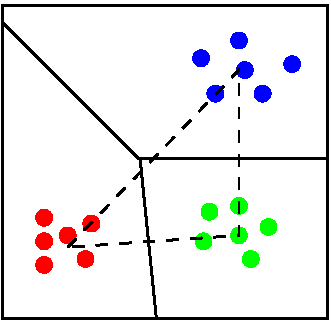
\includegraphics[width=0.5\textwidth]{kmeans-part}
    \caption{Partitioning of data in the $k$-means algorithm.}
    \label{fig:kmeans-part}
  \end{center}
\end{figure}

In the $k-$means methods, the number of clusters to be found is specified by the ``user'', along with the data. The clustering procedure then proceeeds as follows.

\begin{asparaenum}
  \item First, assign every data point to one of the clusters, at random.
  \item Compute the mean position (in the data space) of each cluster by averaging over its assigned members.
  \item For each data point, calculate which of the cluster means it is closest to and re-assign the point to that cluster.
  \item Return to step 2 and repeat until the clusters are not changing.
\end{asparaenum}

This process is illustrated pictorially in Figure~\ref{fig:kmeans}. There are a few points to note:
\begin{asparaitem}
  \item The initial random seeding of the process means that you
  \item The user has to ``guess'' the number of clusters. Too many, and you will split what should be a single cluster. Too few, and you will combine clusters that should be separate, or splitting clusters and merge with others.
  \item This is a computationally ``hard'' algorithm (in the jargon, it is NP-hard). The number of distance calculations increases rapidly with the number of clusters and the number of data points so it can be very costly for large datasets.
  \item Although we have used Euclidean distance in the examples, $k$-mean equally be used with other distance metrics.
  \item Linkage strategies are not required as the only distances computed are between the points and the means.
\end{asparaitem}

\begin{marginfigure}
  \raggedright
  Initial data points

  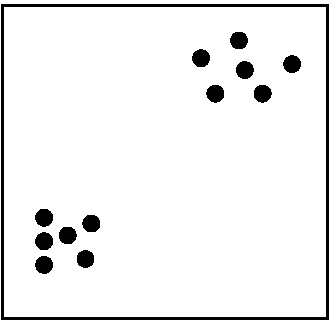
\includegraphics[height=0.12\textheight]{kmeans1}

  Randomly assign points to groups

  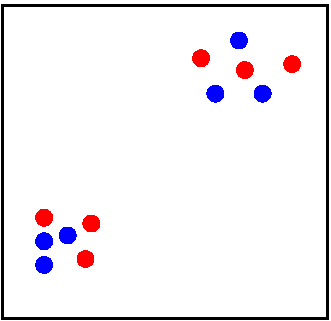
\includegraphics[height=0.12\textheight]{kmeans2}

  Compute group average

  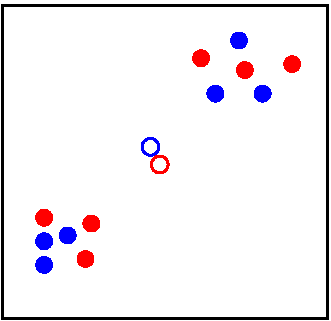
\includegraphics[height=0.12\textheight]{kmeans2av}

  Re-assign points to groups

  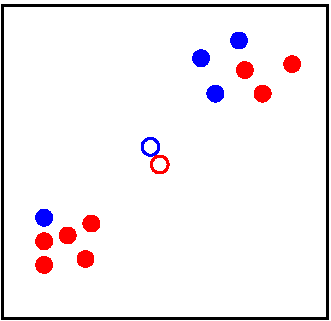
\includegraphics[height=0.12\textheight]{kmeans3}

  Re-compute group averages

  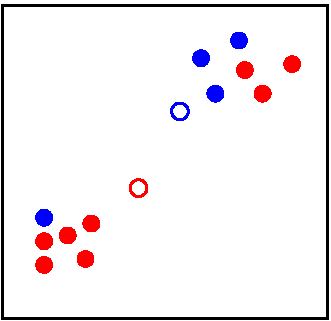
\includegraphics[height=0.12\textheight]{kmeans3av}

  Re-assign points to groups

  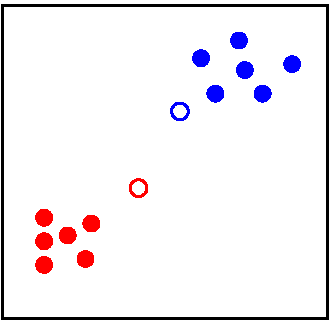
\includegraphics[height=0.12\textheight]{kmeans4}

  Re-compute group averages

  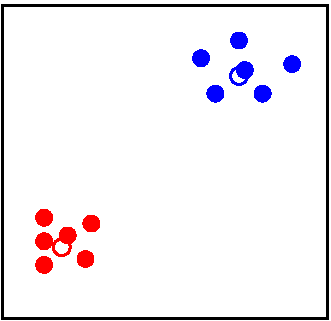
\includegraphics[height=0.12\textheight]{kmeans4av}

  \caption{Illustration of the $k$-means algorithm.}

  \label{fig:kmeans}
\end{marginfigure}

\begin{algorithm2e}[h]
  \SetLine

  \SetKwComment{com}{\% }{}
  \KwData{Data points $Data[N]$; Number of clusters $K$}
  \KwResult{$\bp,e(\bp)$, parameters that minimmise the least squares error, the
 error.}

  \com{Randomly assign each point to a cluster}
  \For{$i\gets 1$ \KwTo $N$}{
    $ClusterIndex[i]\gets randint(1,K)$
  }
  \com{Calculate the mean of each cluster}
  \For{$i\gets 1$ \KwTo $K$}{
    $ClusterMean[i] \gets mean(Data[Cluster[i]])$
  }

  \com{Iterate until clusters are stable}
  $Converged\gets False$\;
  \While{$Converged==False$}{

      \com{Compute distance from every point to each cluster mean}
      \For{$i\gets 1$ \KwTo $K$}{
        \For{$j\gets 1$ \KwTo $N$}{
          $dist[i][j] \gets distance(ClusterMean[i],Data[j])$
        }
      }

      \com{Find the nearest mean for each data point}
      \For{$i\gets 1$ \KwTo $N$}{
        \For{$j\gets 1$ \KwTo $K$}{
          $NewClusterIndex[i] = nearest(Data[i],ClusterMean[j])$
        }
      }

      \com{Generate new clusters}
      \For{$j\gets 1$ \KwTo $K$}{
        $ClusterMean[i] \gets mean(Data[NewClusterIndex==i])$
      }

      \com{Check to see if cluster membership has changed}
      $Converged\gets True$

      \If{NewClusterIndex != ClusterIndex}{
          $Converged \gets False$
      }

      \com{Replace old clusters with new ones}
      $ClusterIndex \gets NewClusterIndex$
      $ClusterMean \gets NewClusterMean$
  }
  \caption{The $k$-Means Algorithm.}
  \label{alg:kmeans}
\end{algorithm2e}

\section{Agglomerative Clustering}
The $k$-means algorithms works by subdividing the whole dataset into ``flat'' subgroups with no internal structure, and if a different number of clusters is required, the algorithm must be re-run. Whilst this is a very popular approach, it is quite limited in terms of the types of clusters it can find: the strict convex partitioning of space it produces is not appropriate for many types of data. Another popular approach that allows some of these problems to be overcome is to build them up (agglomerate) clusters in a hierarchical manner. In this approach, we start by considering the individual data points. We calculate the distance between every pair of points, and group together the pair that are closest. We then remove that pair of points from the list of points, and replace it with the grouped pair. In the next iteration, all distances are again calculated, but this time we must compute the distance to the pairing computed in the first round. This is where the linkage strategies depicted in Figure~\ref{fig:linkage} become relevant: we must decide what distance should be calulated: nearest (single), average of farthest (complete). Again the closest pairing is chosen, removed from the list and replaced with it's group. An example of this is shown in Figure~\ref{fig:hier} and it is instructive to work through it. 
\begin{eqnarray*}
\mbox{List of points}&\mapsto&0,1,2,3,4,5,6\\
\mbox{Group 1 with 2}&\mapsto&0,3,4,5,6,(1,2)\\
\mbox{Group 3 with 4}&\mapsto&0,5,6,(1,2),(3,4)\\
\mbox{Group 0 with (1,2)}&\mapsto&5,6,(3,4),(0,(1,2))\\
\mbox{Group 5 with 6}&\mapsto&(3,4),(0,(1,2)),(5,6)\\
\mbox{Group (3,4) with (0,(1,2))}&\mapsto&(5,6),((3,4),(0,(1,2)))\\
\mbox{Group (5,6) with ((3,4),(0,(1,2)))}&\mapsto&((5,6),((3,4),(0,(1,2))))
\end{eqnarray*}

The most common way to represent this is with the \textbf{dendrogram} shown in Figure~\ref{fig:hier}. The height of each ``junction'' in the dendrogram represents the distance between the points being paired (so $(3,4)$ join at height 1, for example).

\begin{figure*}
  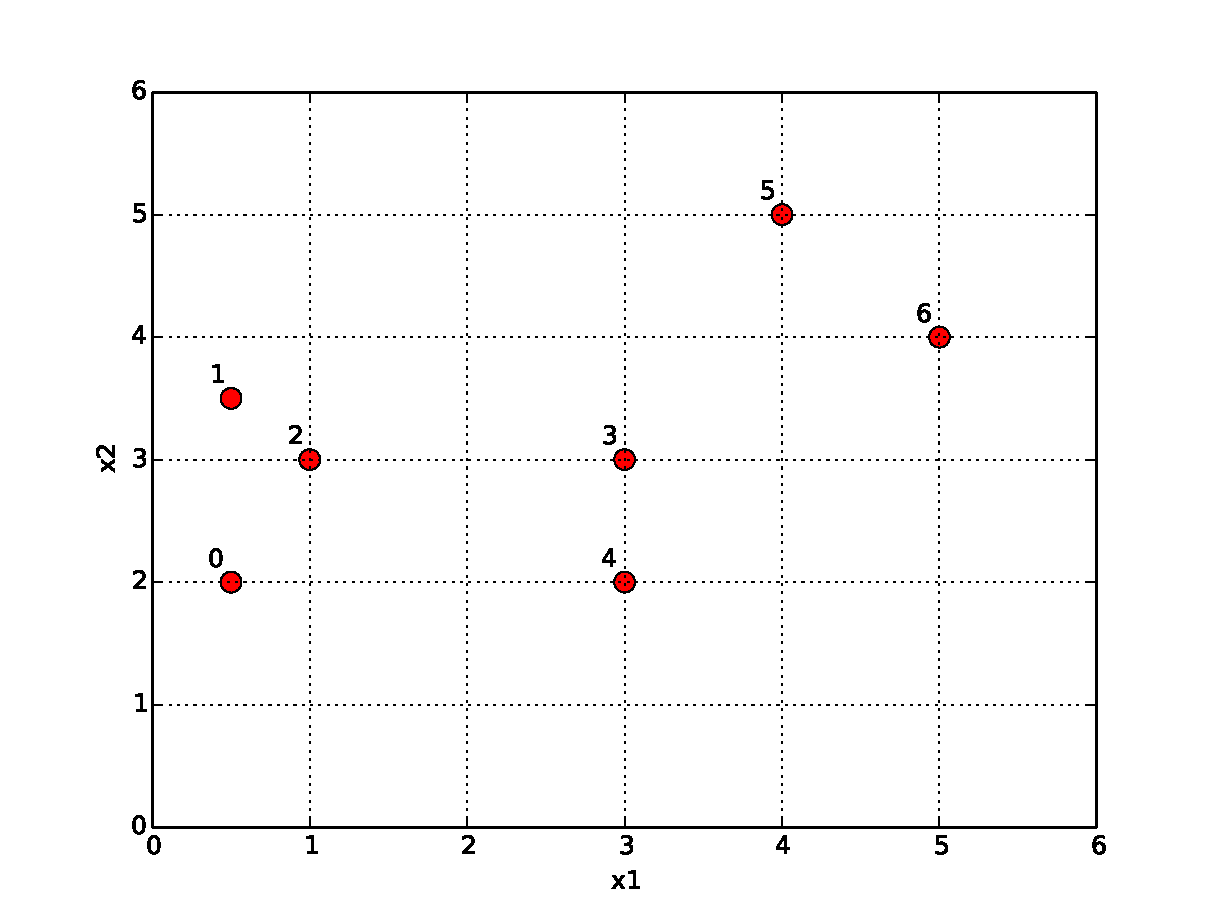
\includegraphics[width=0.5\textwidth]{hierpts}
  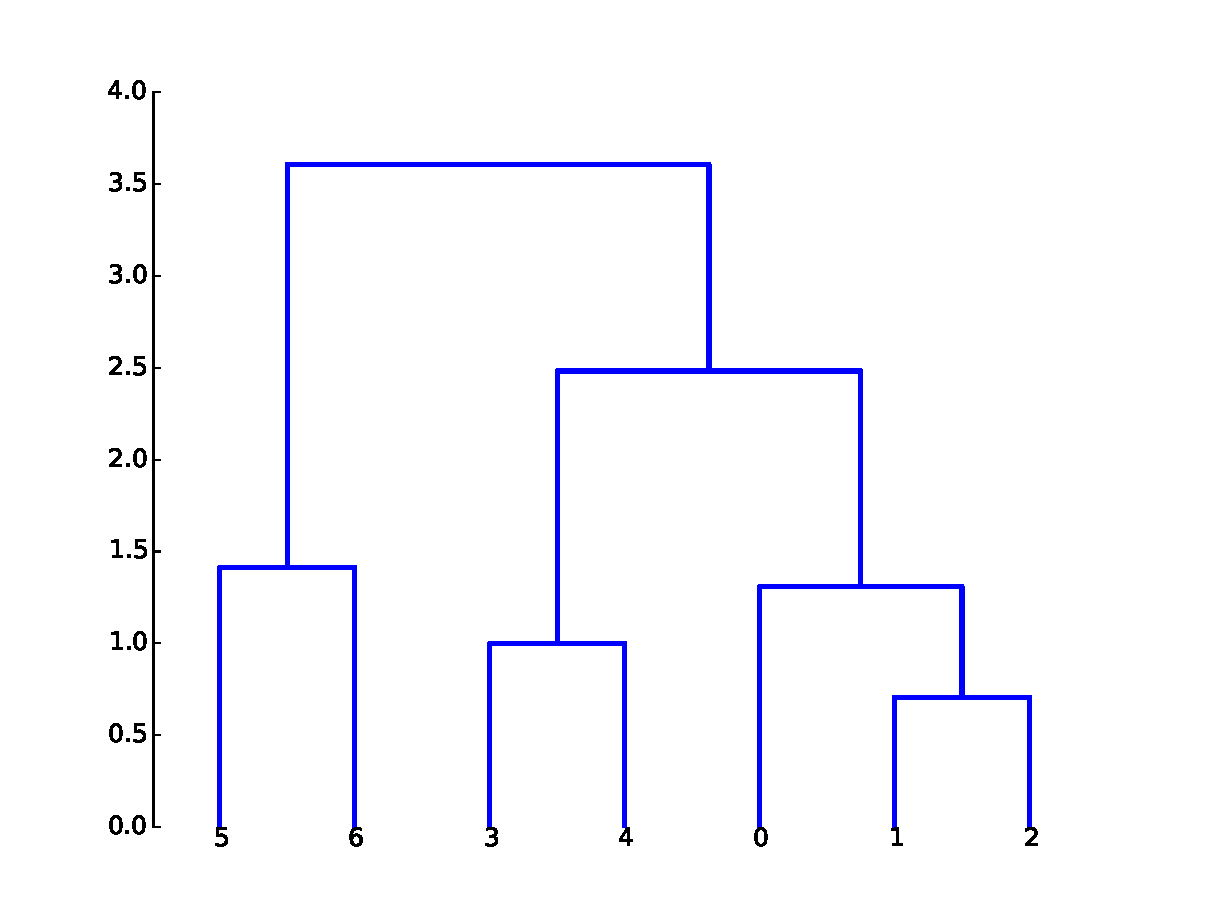
\includegraphics[width=0.5\textwidth]{dendro}
  \caption{Datapoints for Hierachical Clustering and the resulting dendrogram using euclidean distance with average linkage.}
  \label{fig:hier}
\end{figure*}

One of the advantages of this methods is that it generates all numbers of clusters. By cutting horizontally across the dendrogram at different heights we can obtain the desired number of clusters just by choosing how many lines we cut. The disadvantage is that it can be very time consuming to compute the dendrogram: if there are a large number of sample points, and pairwise distance calulations have to be done between all of them in the first instance, then this very quickly becomes computationally expensive. Compare this to $k$-means, where the distance calulation is between the $N$ points and the $K$ cluster centres: $N\times K$ evaluations of the distance function vs the $\frac{n!}{k!\,(n-k)!}$ calculations needed just to compute the first pairing.

\section{Other Clustering Methods}
These are but two of the available clustering techniques, but they are two of the most commonly used. Even so, there are still many free choices:
\begin{asparaitem}
  \item How many clusters?
  \item Which distance metric?
  \item What linkage method?
\end{asparaitem}

To find the combination that is optimal for a given experiment is often a matter of trial-and-error. It is, however, important to understand how these algorithms work so that you can understand the underlying assumptions. Understanding how the $k$-means algorthm partitions space, for example, allows you to realise that concave clusters or those of very different sizes not not be correctly separated. No single technique is suited for all problems and you must understand both the problem, and the assumptions in the algorithms to understand what types of clusters will be found by these methods.

We have only looked in detail at two clustering methods and many other clustering tools are available. Matlab Statistics Toolbox includes some of them, but a much more comprehensive suite of modern clustering tools is provided by the ELKI (Environment for Developing KDD-Applications Supported by Index-Structures) package which is available from \url{http://elki.dbs.ifi.lmu.de/}. This software includes modern techniques such as the OPTICS\citep{ankerst1999optics} and DBSCAN\citep{ester1996density} algorithms that perform density-based clustering.

\bibliographystyle{alpha}
\bibliography{clustering}




\end{document}
